\section{External interface requirements}

\subsection{User interfaces}
Here we show some mockups of the user interface. These screens are aimed at
giving an overview of how the interface for the main functions should look like.
However the final implementation may differ from this.

As stated earlier in section \vref{sec:ass_deps_constr} the user (i.e.\
citizen) will access the service through a mobile application. The mockups
of the app screens are shown in figure \vref{fig:mockups_mobile}.
The operators, on the other hand, will access the service through a web portal,
whose pages are represented in figure \vref{fig:mockups_web}. Note that the
suggestion function will only be displayed if \emph{SmartSuggestions} is active
for that particular authority.

% Mobile user interface
\begin{figure}[h]
    \centering
    \begin{subfigure}{0.3\textwidth}
        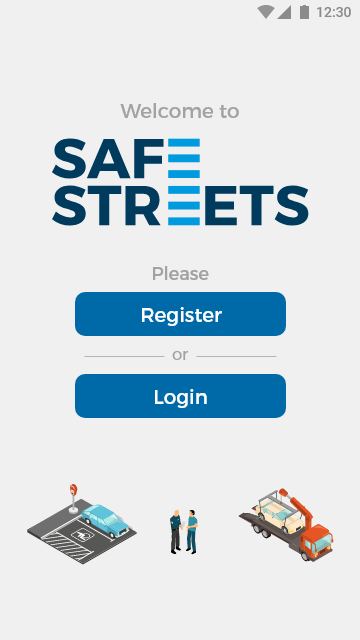
\includegraphics[width=\textwidth]{mobile_landing}
        \caption{Landing page}
    \end{subfigure}
    ~
    \begin{subfigure}{0.3\textwidth}
        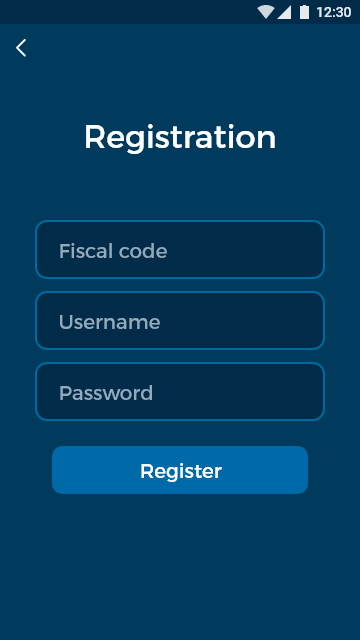
\includegraphics[width=\textwidth]{mobile_registration}
        \caption{Registration page}
    \end{subfigure}
    ~
    \begin{subfigure}{0.3\textwidth}
        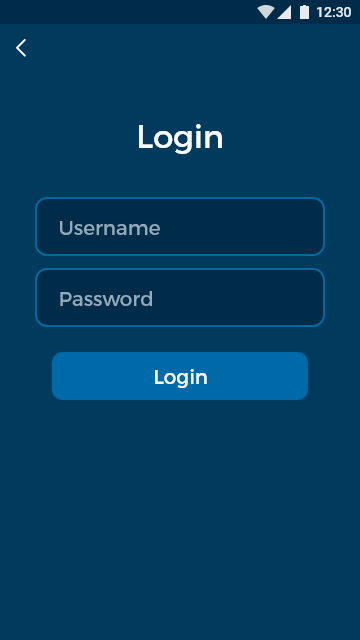
\includegraphics[width=\textwidth]{mobile_login}
        \caption{Login page}
    \end{subfigure}

    \caption{Mockups of the mobile interface, used by the citizens}
    \label{fig:mockups_mobile}
\end{figure}%
\begin{figure}[ht]\ContinuedFloat
    \centering
    \begin{subfigure}{0.3\textwidth}
        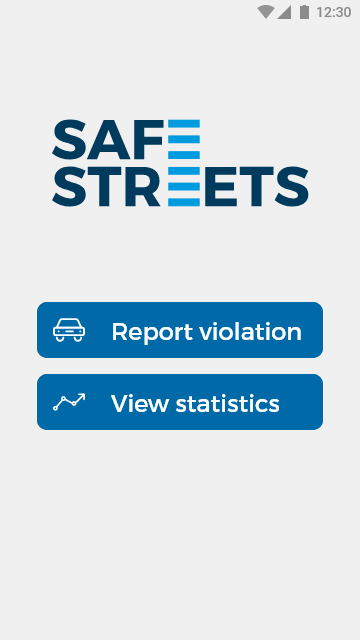
\includegraphics[width=\textwidth]{mobile_menu}
        \caption{Main menu}
    \end{subfigure}
    ~
    \begin{subfigure}{0.3\textwidth}
        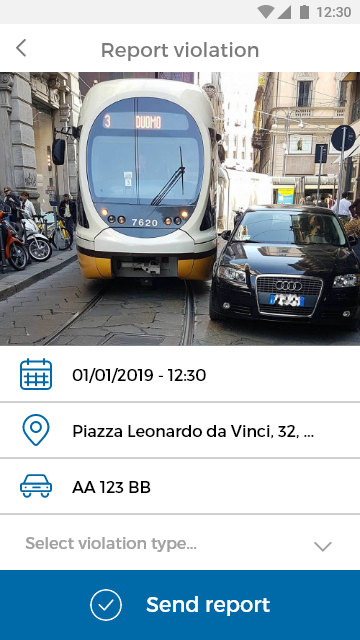
\includegraphics[width=\textwidth]{mobile_report}
        \caption{Violation reporting page}
    \end{subfigure}

    \begin{subfigure}{0.3\textwidth}
        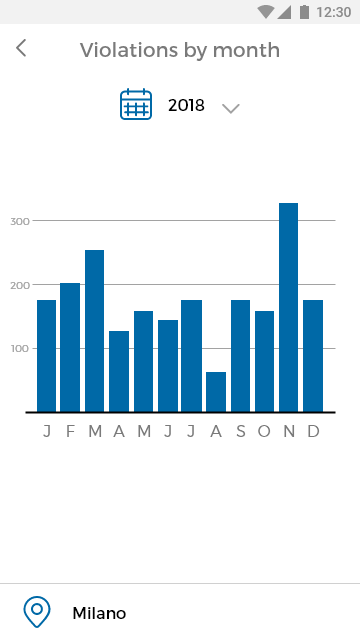
\includegraphics[width=\textwidth]{mobile_statistics_histogram}
        \caption{Statistics page: histogram}
    \end{subfigure}
    ~
    \begin{subfigure}{0.3\textwidth}
        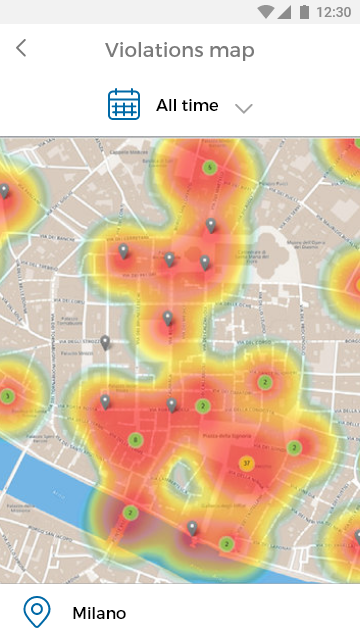
\includegraphics[width=\textwidth]{mobile_statistics_map}
        \caption{Statistics page: heat map}
    \end{subfigure}
    
    \caption{Mockups of the mobile interface, used by the citizens}
\end{figure}

% Web user interface
\begin{figure}[ht]
    \centering
    \begin{subfigure}{\textwidth}
        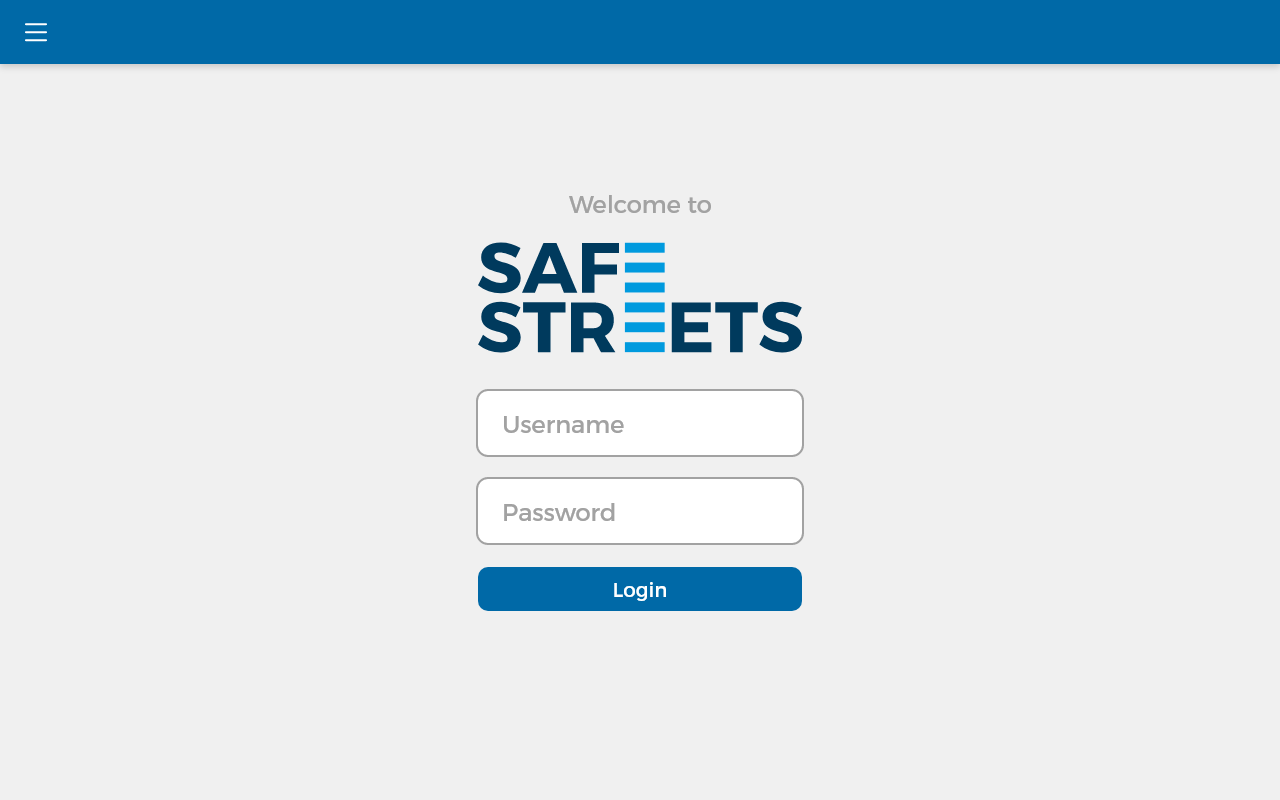
\includegraphics[width=\textwidth]{web_landing}
        \caption{Landing page}
    \end{subfigure}

    \begin{subfigure}{\textwidth}
        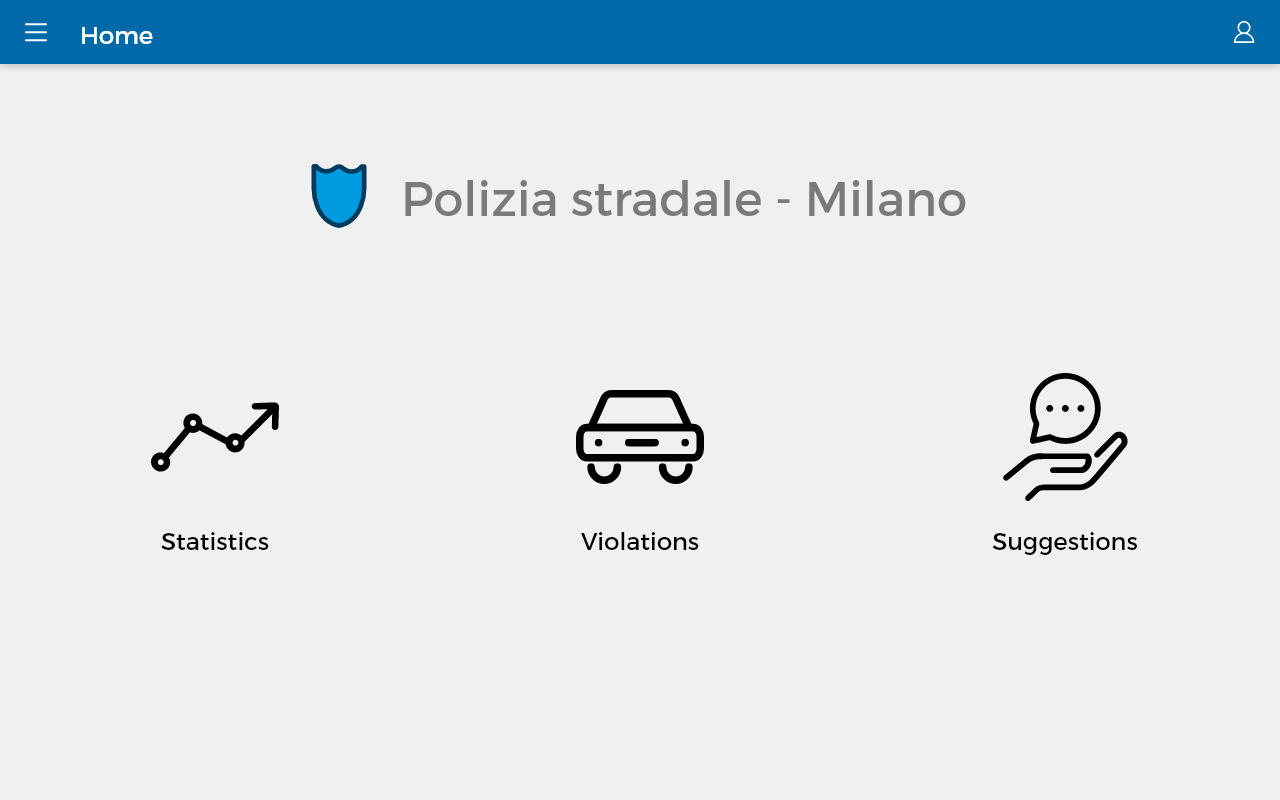
\includegraphics[width=\textwidth]{web_home}
        \caption{Main menu}
    \end{subfigure}

    \caption{Mockups of the web interface, used by the authority operators}
    \label{fig:mockups_web}
\end{figure}
\begin{figure}[ht]\ContinuedFloat
    \centering
    \begin{subfigure}{\textwidth}
        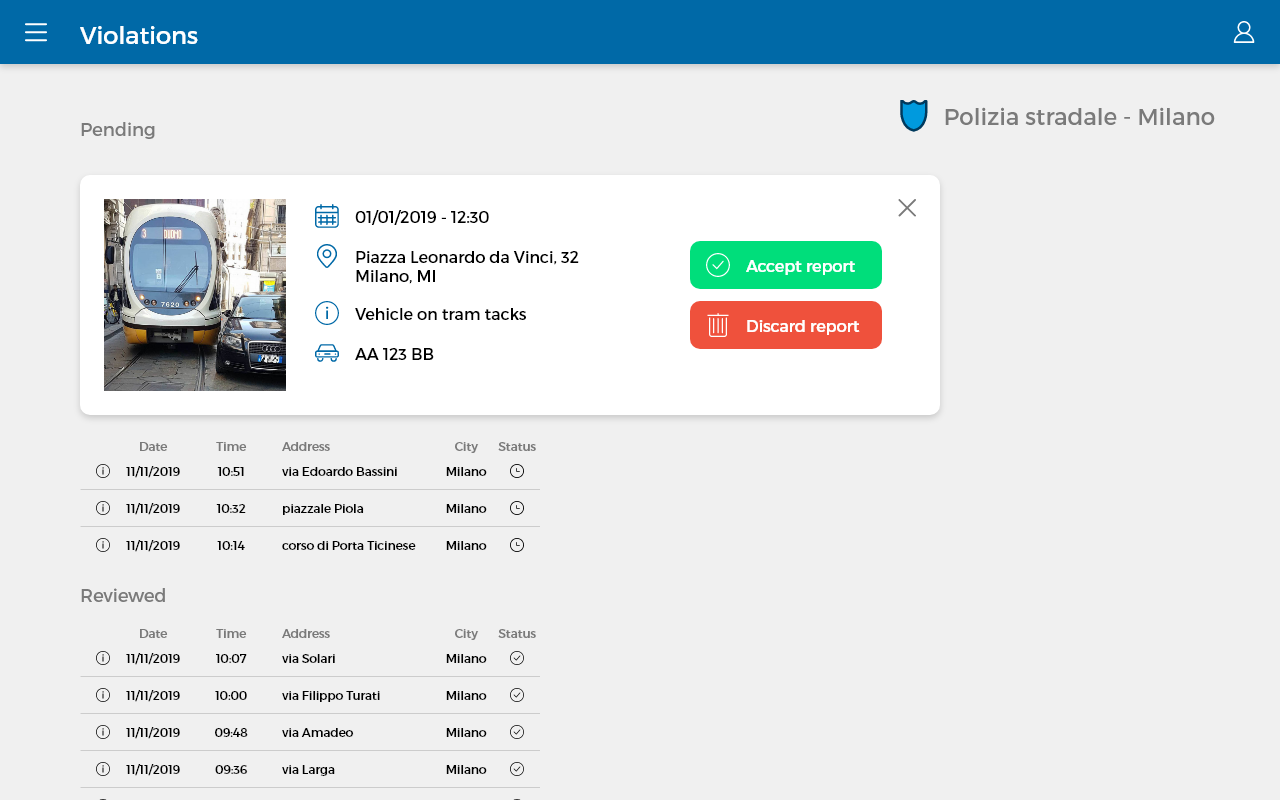
\includegraphics[width=\textwidth]{web_violations}
        \caption{Violations list}
    \end{subfigure}
    
    \begin{subfigure}{\textwidth}
        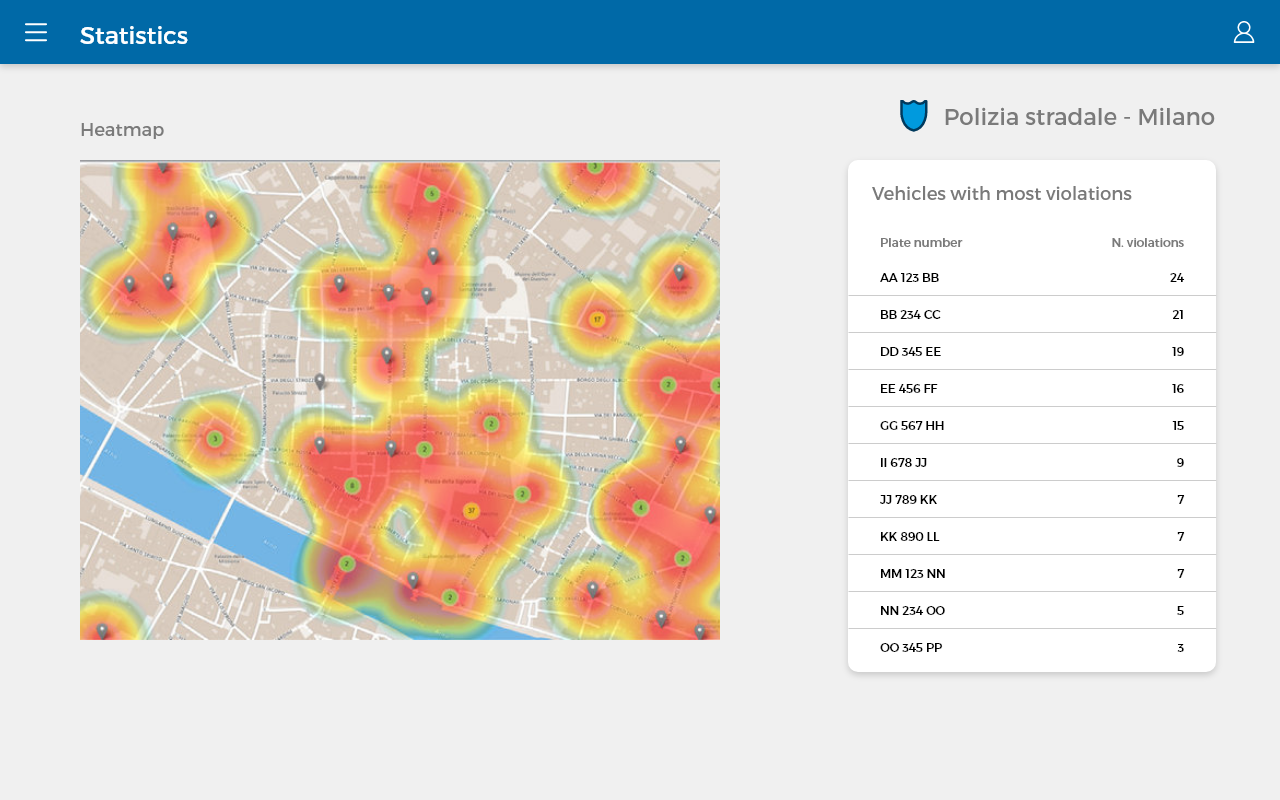
\includegraphics[width=\textwidth]{web_statistics}
        \caption{Statistics page}
    \end{subfigure}

    \caption{Mockups of the web interface, used by the authority operators}
\end{figure}
\clearpage % Allow figures to be printed
\begin{figure}[ht]\ContinuedFloat
    \centering
    \begin{subfigure}{\textwidth}
        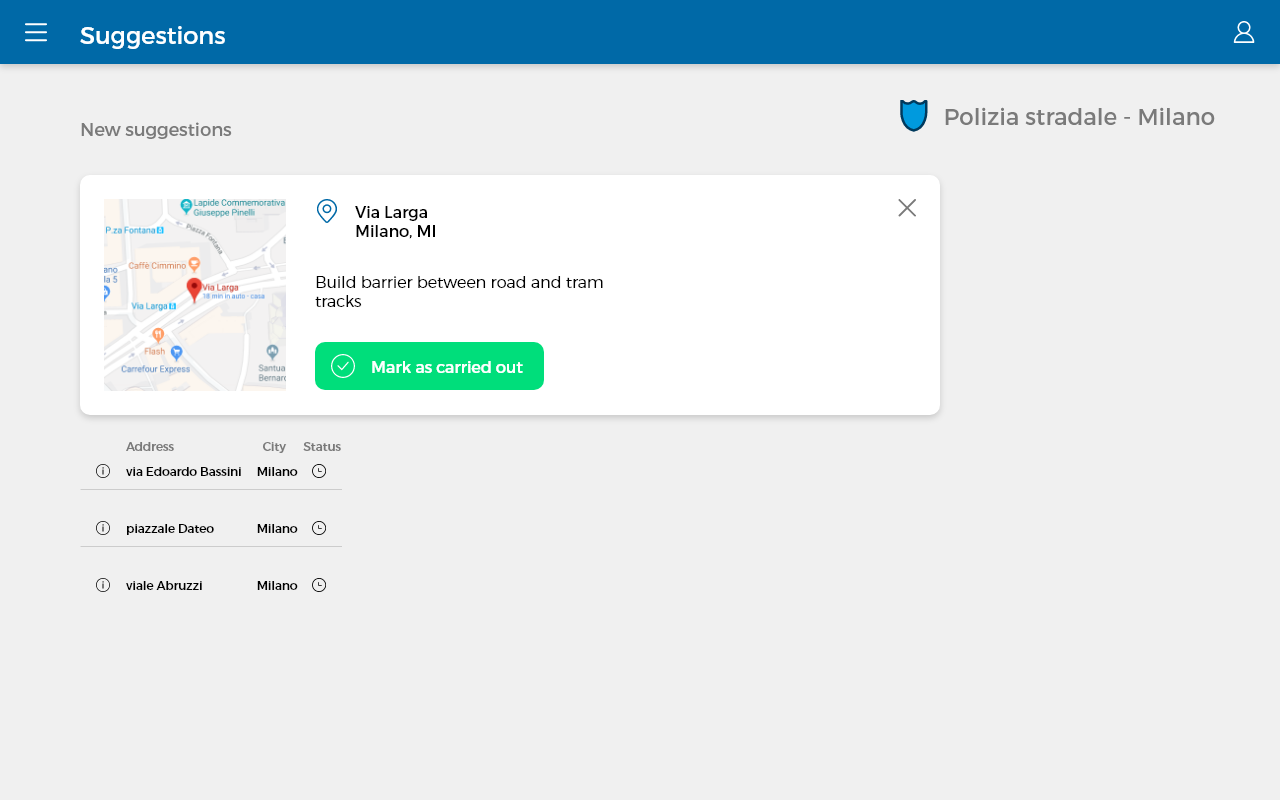
\includegraphics[width=\textwidth]{web_suggestions}
        \caption{Suggestions page}
    \end{subfigure}

    \caption{Mockups of the web interface, used by the authority operators}
\end{figure}

\subsection{Hardware interfaces}
The system doesn't provide any hardware interfaces.

\subsection{Software interfaces}
The S2B doesn't provide any external API: the service is accessible only
from the user interface.
However, the implementation will most likely use an internal API to allow
interaction between components.
In case the authority will need to integrate the S2B with other systems, some
time in the future, this internal API might be standardized and made available
to the authority.

\subsection{Communication interfaces}
The S2B uses the internet as the standard communication facility.
No other communication interfaces are planned.